\apendice{Plan de Proyecto \textit{Software}}

\section{Introducción}

En este anexo, se incluye la planificación temporal, económica y la viabilidad legal de este trabajo. La planificación temporal, engloba tanto las distintas fases del proyecto (o \textit{sprints}) como algunos de los inconvenientes que han surgido durante su desarrollo. En el caso de la planificación económica, se muestra el coste aproximado del proyecto en un periodo de 6 meses. Y, por último, en la viabilidad legal, se analizan las normativas que deben cumplirse para su correcta implementación.

\section{Planificación temporal}

Este TFG comenzó el 15 de diciembre de 2023 en una reunión con los tutores para empezar a realizar las primeras tareas, las cuales están indicadas en GitHub, en el \textit{milestone} ``Comenzar con el TFG''.

En ese momento el tema de este TFG era distinto al actual ya que, debido a diversos factores, se han tenido que realizar algunos cambios en el tema del TFG, hasta que, finalmente se ha podido realizar este.

En un principio, el tema del TFG fue ``Estadiaje de cáncer de pulmón mediante aprendizaje automático a partir de imágenes'', es decir, identificación de la existencia de cáncer de pulmón en imágenes de TAC de pacientes del HUBU empleando redes neuronales. Pero, tras una segunda tutoría, esta vez en el hospital, donde se estuvo en contacto con los médicos que iban a proporcionar dichas imágenes, se llegó a la conclusión de que no era viable trabajar con imágenes de TAC dada su complejidad. Ya que, al ser imágenes tridimensionales donde, existen múltiples cortes de la misma zona, la cantidad de datos a procesar aumenta considerablemente. Además, se debe analizar cada uno de los cortes individualmente, lo cual, representa un desafío técnico considerable. Por lo tanto, tras esta tutoría se asignó un nuevo TFG.

En este segundo TFG, la idea era emplear imágenes de CXT asociadas a un posible cáncer de pulmón de los pacientes del HUBU, las mismas imágenes que emplearía mi compañero Roberto Martínez-Guisasola Guerrero, pero, con un propósito distinto. El objetivo de este TFG era identificar cáncer de pulmón a partir de las imágenes mencionadas previamente implementando una red neuronal capaz de determinar la presencia de cáncer y señalar el lugar exacto del tumor. Esto se conseguía realizando una anotación previa de cada una de las imágenes con ayuda de un neumólogo especializado. Esta anotación consistía en, empleando un \textit{software} específico, se delimitaba en cada una de las imágenes el tumor o, en su defecto, ausencia de tumor, delimitando todo el tórax.

Pero, para comenzar a trabajar con estas imágenes era necesaria una previa aprobación por parte del comité de bioética para proteger la identidad y privacidad de los pacientes. Por lo que, tanto mi compañero Roberto como yo, tuvimos que redactar un informe al comité de bioética para presentar a fecha de 19 de febrero de 2024. Mientras se realizaba dicho informe y se esperaba a su posible aprobación o desaprobación, se realizaron otra serie de tareas indicadas en GitHub en el \textit{milestone} ``Pautas a realizar tras la tercera reunión de TFG 2/02/2024''. Entre estas tareas, cabe destacar la visualización y aplicación del video ``Real Time Face Mask Detection with Tensorflow and Python | Custom Object Detection w/ MobileNet SSD'' \footnote{\url{https://www.youtube.com/watch?v=IOI0o3Cxv9Q}} ya que, supuso bastantes problemas relacionados con el entorno de Anaconda y las versiones por lo que, se tardó mucho más tiempo del que debería. Aunque, finalmente, lo indicado en este video no fue necesario para la realización de este TFG ya que, por tercera vez se tuvo que volver a cambiar de tema.

A principios de marzo, el comité de bioética denegó la solicitud por lo que, si se quería volver a presentar, antes se tenía que realizar algún cambio. Tras considerar diversas opciones, se llegó a la conclusión de que, esperar a una posible aprobación por parte del comité de bioética suponía una pérdida de tiempo muy valioso en el desarrollo del TFG. Por lo tanto, se optó por realizar un cambio en el enfoque del TFG. 

Esta tercera y última opción consiste en, identificar una posible neumonía en imágenes de CXT obtenidas de internet implementando una red neuronal profunda. A partir de la tutoría del día 21 de marzo de 2024, se comenzó a trabajar en este TFG definitivo indicando un ``\textit{milestone}'' (o hito) por cada reunión que se ha tenido. Dentro de cada ``\textit{milestone}'' aparecen las tareas propuestas a realizar tras cada reunión.

Mencionar que, en un principio no se sabía muy bien como había que utilizar GitHub ya que, inicialmente se intentó trabajar con ZenHub, una herramienta de gestión de proyectos ágil asociada a  GitHub pero, después de mucho investigar se concluyó que, se había acabado el plazo para solicitar las plazas gratuitas para estudiantes durante un año y, ya no se disponía de acceso gratuito a esta opción por lo que, se barajaron otras herramientas como ``Asana'' o ``Jira'' pero, después de probarlas, la conclusión acabó siendo la misma y es que, había la opción gratuita durante un mes pero después, o se pagaba o las condiciones cambiaban por lo que, también se descartaron. Tras preguntar al coordinador de TFG, este indicó que, en este grado era suficiente con emplear GitHub y sus correspondientes ``\textit{milestones}'', ``\textit{issues}'' (tareas) y ``\textit{labels}'' (etiquetas). Pero, cuando llego el momento de comenzar a trabajar con GitHub y, hasta que se recordaron las nociones aprendidas en el grado y se dominó correctamente esta plataforma ya se habían realizado varias de las tareas. Por esta razón, GitHub indica un comienzo de trabajo más tardío al que realmente fue y, existen \textit{milestones} y tareas creadas y cerradas al momento (debido a que ya estaban realizadas).

Por otro lado, no se ha comenzado a trabajar con ``GitHub Desktop'' hasta empezar con el TFG definitivo y, después de algún que otro problema ya que, inicialmente no se utilizó correctamente. Por esa razón, aunque, ya se había trabajado con código de Python en el video mencionado previamente (de la segunda opción de TFG), esto no ha quedado reflejado. De todas formas, con este video se tuvo que instalar y desinstalar varias veces tanto el entorno de anaconda con el que se estaba trabajando como la aplicación de Python en sí y tampoco sirve para este TFG. Se comenzó a trabajar con código del TFG definitivo a partir de la tutoría del 21 de marzo, aunque, no se refleja en GitHub hasta principios de abril, momento en el cual, se adquirió un mayor entendimiento sobre el manejo de GitHub Desktop. Cada vez que se ha completado una tarea específica relacionada con código, se ha realizado un commit en GitHub Desktop vinculándolo con la tarea correspondiente para mantener un registro detallado del progreso y las modificaciones en el código.

También hay que tener en cuenta que, tal y como se ha indicado en GitHub, la redacción de la memoria se comenzó previamente a crear el \textit{milestone} ``Redacción de la memoria'' ya que, dentro de otros \textit{milestones} asociados a cada reunión ya existen tareas relacionadas con la redacción de la memoria. 

El \textit{milestone} de ``Lecturas bibliográficas neumonía'' y ``Lecturas bibliográficas neumonía con \textit{deep learning}'' hacen referencia a la lectura de los artículos para la posterior redacción del estado del arte acorde a esos artículos. Lo mismo sucede con el \textit{milestone} ``Lecturas bibliográficas redes neuronales'', el cual se refiere a la lectura del libro para adquirir conocimientos y aportar información en diversas secciones de la memoria, sobre todo en el apartado de ``\textit{Conceptos teóricos}''.

La fecha de vencimiento indicada en algunos \textit{milestones} de las reuniones, se refiere a una fecha orientativa para la realización de las tareas indicadas, generalmente dos semanas, pero, aunque se hubieran realizado todas las tareas, el cerramiento de las ``\textit{issues}'' y ``\textit{milestones}'' no se llevaba a cabo hasta la siguiente tutoría por si quedaba alguna duda relacionada con esas tareas o algo no estaba completo.

Tras esta extensa explicación de la planificación indicada en GitHub y todos los problemas que han surgido, se puede decir que la planificación seguida ha sido la siguiente:

\textbf{\textit{Sprint} 1: ``Comenzar con el TFG'' del 15/12/23 al 24/1/24} 
\begin{itemize}
    \item Descargar y empezar a trabajar con la plantilla de LaTex
    \item Visualización del video colgado en ubuvirtual acerca de los distintos puntos a tener en cuenta en el TFG
    \item Crear repositorio en GitHub
    \item Empezar a trabajar con keras y MNIST desde Python
    \item Hacer una primera revisión para buscar información del cáncer de pulmón en artículos, en la OMS, etc.
    \item Rellenar la solicitud para el acceso a SCAYLE
\end{itemize}

\textbf{Nota 1:} Este \textit{sprint} tiene una duración de más de un mes debido a que coincidió con todos los exámenes finales del primer semestre.

\textbf{Nota 2:} la tarea de ``Crear repositorio en GitHub'', lleva consigo algunos problemas mencionados previamente y por eso, este primer \textit{sprint} no se creó hasta el 18 de febrero en GitHub

\textbf{\textit{Sprint} 2: ``Redefinición TFG'' del 29/1/24 al 18/2/24}
\begin{itemize}
    \item Realización del informe de solicitud para el comité de bioética 
\end{itemize}

\textbf{\textit{Sprint} 3: ``Pautas a realizar tras la tercera reunión de TFG 2/02/2024'' del 2/2/24 al 13/3/24}
\begin{itemize}
    \item Visualización del video ``Real Time Face Mask Detection with Tensorflow and Python | Custom Object Detection w/ MobileNet SSD'' \footnote{\url{https://www.youtube.com/watch?v=IOI0o3Cxv9Q}} para realizarlo en un script de Python
    \item Crear un nuevo entorno virtual en anaconda para trabajar en el TFG
    \item Investigar como trabajar con la plantilla de overleaf (LaTex)
    \item Comenzar a leer el libro ``Fundamentos de visión por computador'' para entender mejor algunos conceptos importantes para este trabajo y para servir de ayuda en la redacción de la memoria
\end{itemize}

\textbf{Nota 1:} Este \textit{sprint} se solapa con el anterior debido a que, el anterior pertenece a la tutoría realizada en el hospital donde se indicó esa tarea a realizar y, se acordó una nueva tutoría para poder avanzar con otras tareas a la vez que se realizaba el informe.

\textbf{Nota 2:} Como ya se ha comentado previamente, la visualización de este video, supuso una serie de problemas por lo que, en este periodo de tiempo se solicitaron varias tutorías para solucionar cada uno de los problemas que iban surgiendo pero, no se indicaban nuevas tareas y, por tanto no se visualizan como nuevos \textit{sprints}.

\textbf{\textit{Sprint} 4: ``Reunión 13/3/24'' del 13/3/2024 al 21/3/24}
\begin{itemize}
    \item Comenzar a trabajar con GitHub Desktop
\end{itemize}

\textbf{Nota 1:} Esta reunión no está reflejada en GitHub debido a que fue en medio de todo el proceso de cambio de TFG dónde no se sabía cuál iba a ser el TFG definitivo y, por lo tanto no habían tareas claras a realizar hasta que esto no se decidiera. Además, aunque a partir de esta reunión se comenzó a trabajar con GitHub Desktop, no fue hasta un par de tutorías más tarde que, se empezó a trabajar de la forma correcta con esta herramienta. 

\textbf{Nota 2:} A partir del siguiente \textit{Sprint} ya se empieza a trabajar con el TFG definitivo

\textbf{\textit{Sprint} 5: ``Primera reunión con el TFG definitivo 21/03/2024'' del 21/3/24 al 8/4/24}
\begin{itemize}
    \item Modificar el código de MNIST sacado de internet para acceder a imágenes ya descargadas en lugar de imágenes de internet.
    \item Modificar el código de MNIST sacado de internet para un problema de clasificación binaria
    \item Comprobar que el código funciona correctamente entrenando 10 épocas y calcular una serie de métricas como \textit{accuracy}, sensibilidad, sensitividad, AC o F1.
\end{itemize}

\textbf{\textit{Sprint} 6: ``Reunión TFG 8/4/24'' del 8/4/24 al 3/5/24}
\begin{itemize}
    \item Investigar acerca del parámetro callback (\textit{Early Stopping}) y añadirlo en la parte de conceptos teóricos de la memoria
    \item Modificar parámetros de la función model.fit (para entrenar el modelo), añadiendo el callabck (\textit{Early Stopping})
    \item Realización de métricas a mano en lugar de, automáticamente con keras
    \item Crear distintos modelos con distintas arquitecturas (Simple1, Simple2...), variando el número de neuronas/capas para comparar los resultados con un determinado \textit{batch size}.
    \item Investigar acerca del valor de \textit{batch size} en \textit{train} y como este afecta en el resultado y añadirlo en la parte de conceptos teóricos de la memoria
    \item Probar distintos valores de \textit{batch size} para las distintas arquitecturas realizadas previamente
    \item Comparación de las distintas arquitecturas para distintos \textit{batch size} y escoger la mejor opción en cuanto a métricas
    \item Realización en Python (u otro programa) de tablas y/o gráficas para visualizar los resultados de las métricas para las distintas arquitecturas en distintos \textit{batch size}
    \item Comenzar con la lectura de los artículos indicados en el milestrone ``Lecturas bibliográficas neumonía'' para la redacción del estado del arte de la memoria
    \item Comenzar a redactar tanto el resumen como la introducción 
\end{itemize}

\textbf{Nota:} La redacción del resumen y la introducción, no está indicada en el \textit{milestone}  porque, en un principio no era una tarea de este \textit{sprint} pero, una vez se empezó a redactar en la memoria, se decidió comenzar con estos dos puntos.

\textbf{\textit{Sprint} 7: ``Reunión TFG 3/5/24'' del 3/5/24 al 16/5/24}
\begin{itemize}
    \item Volver a intentar la realización de todas las métricas a mano ya que en el \textit{sprint} anterior solo se acabaron consiguiendo unas pocas.
    \item Modificación del código realizado previamente para adaptarlo a estas nuevas métricas
    \item Analizar los resultados obtenidos. Redactar en la memoria la comparativa de las tablas/gráficas y el porqué de los resultados obtenidos.
    \item Explicar en la parte de ``metodología'' de la memoria cómo se va a trabajar con las diferentes tablas (en este caso \textit{batch size} y \textit{EarlyStopping})
    \item Una vez elegida la mejor arquitectura y el mejor \textit{batch size}, se prueban distintos valores de neuronas (32, 64, 128, 156) para la capa o capas ocultas y se selecciona la mejor opción.
    \item Analizar en el apartado de ``Resultados'' de la memoria, los resultados obtenidos con distintos valores de neuronas
    \item Explicar en la parte de ``Metodología'' de la memoria cómo se va a trabajar con la tabla donde se compara el número de neuronas.
    \item Redactar en el apartado de ``Conceptos teóricos'' información acerca de redes neuronales, aprendizaje automático y aprendizaje profundo.
    \item Redacción del estado del arte a partir de los artículos del \textit{milestone} ``Lecturas bibliográficas neumonía'' y ``Lecturas bibliográficas neumonía con \textit{deep learning}''
    \item Avanzar en otros puntos de la memoria como conceptos teóricos y objetivos
\end{itemize}

\textbf{\textit{Sprint} 8: ``Reunión TFG 16/5/24'' del 16/5/24 al 24/5/24}
\begin{itemize}
    \item Comenzar a redactar el anexo de planificación e incluir en el apartado de ``\textit{Aspectos relevantes}'' de las conclusiones, todos los inconvenientes que han surgido durante la realización de este trabajo
    \item Modificación de la bibliografía para solucionar algunos errores
    \item Modificar el número de épocas a 20 en las tablas realizadas previamente para poder observar mejores resultados
    \item Modificar las tablas realizadas previamente eliminando el índice, y redondeando los decimales de la tabla a 2 para que se puedan visualizar mejor los resultados en el documento.
    \item Tras cambiar el número de épocas, puede que los resultados cambien, por lo tanto, si esto sucede, se deben modificar los resultados en la memoria.
    \item Revisar y dejar correctamente escrito toda la parte de introducción, resumen, conceptos teóricos escritos hasta ahora, estado del arte, parte de la metodología redactada hasta ahora y parte de los resultados redactados hasta ahora.
\end{itemize}

\textbf{\textit{Sprint} 9: ``Reunión TFG 24/5/24'' del 24/5/24 al 3/6/24}
\begin{itemize}
    \item Realización de una función para dividir el número de imágenes de forma correcta ya que, tal y como están distribuidas las imágenes en el dataset original se complica la obtención de buenos resultados.
    \item Redactar en el apartado de ``\textit{Descripción de los datos}'' la nueva división de imágenes.
    \item Modificar parámetros y averiguar por qué no se obtienen buenos resultados en las tablas comparativas realizadas previamente
\end{itemize}

\textbf{\textit{Sprint} 10: ``Reunión TFG 3/6/24'' del 3/6/24 al 17/6/24}
\begin{itemize}
    \item Modificación y ejecución de código para ver si los resultados de las tablas mejoran ya que, los resultados obtenidos continúan siendo malos sin explicación alguna. Esto incluye la creación de la CNN AlexNet para hacer las correspondientes comparaciones.
    \item Creación de gráficas para visualizar el rendimiento del modelo en el entrenamiento y la validación y explicar estos resultados en la memoria
    \item Realizar modificaciones en la memoria y anexos (sobre todo en la parte más biológica) acorde al feedback recibido tras el envío del primer borrador de la memoria.
    \item Completar toda la información tanto en la memoria como en los anexos para poder enviar el primer borrador completo del TFG a ambos tutores.
    
    

\end{itemize}

\textbf{\textit{Sprint} 11: ``Reunión TFG 17/6/24'' del 17/6/24 al 28/6/24}
\begin{itemize}
    \item Para que se guarden los modelos que se ejecutan tras cada entrenamiento y, así poderse reutilizarlos en caso necesario (como para la creación de la matriz de confusión), se ha de añadir ``model.save'' y, después ``model.load'' para recuperar el modelo
    \item Modificar memoria y anexos acorde a los nuevos resultado
    \item Completar el apartado ``Pruebas del sistema'' dentro del anexo manual del programador
    \item Crear una carpeta ``resultados'' con python donde se encuentren todos los csv de los históricos para que estén más ordenados
    \item Añadir todas las carpetas/documentos empleados en este trabajo en el repositorio de GitHub
    \item Ejecutar notebook del archivo.py
    \item Rematar todos los anexos y memoria para poder entregar un borrador a los tutores
\end{itemize}

Para concluir, en la figura \ref{fig:grafica_planificacion} se muestra gráficamente el ritmo de trabajo llevado a cabo durante este proyecto. En esta gráfica, se pueden observar dos picos significativos en la actividad, uno al inicio y otro al final. Y es que, tal y como se ha comentado previamente, GitHub se comenzó a usar posteriormente al comienzo del proyecto por lo que, todas las tareas que ya se habían realizado previamente se tuvieron que abrir y cerrar al momento. Por otro lado, el pico final, se corresponde con la redacción y revisión final de cada uno de los apartados de la memoria y los anexos. Y, dado que estas revisiones se estuvieron realizando hasta el último momento, las tareas se han cerrado de forma simultánea al finalizar el proyecto.

\begin{figure}[h]
        \centering
        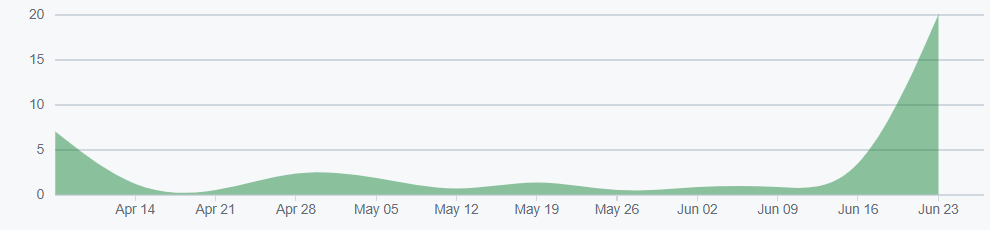
\includegraphics[width=0.99\textwidth]{img/grafica_planificacion.PNG}
        \caption{Contribución de las tareas realizadas con GitHub. Fuente propia.}
        \label{fig:grafica_planificacion}
    \end{figure}

\subsection{Planificación económica}

Los costes se van a calcular sobre un periodo aproximado de 6 meses tanto a nivel de personal como de \textit{hardware} y de \textit{software}.

\subsubsection{Personal}

Aunque el salario de un ingeniero es mayor que el salario mínimo mensual, en este caso se va a calcular la planificación económica a nivel de personal con esa referencia para conseguir un coste aproximado. Tabla \ref{tab:personal}.

El salario mínimo mensual neto en 2024 es de 1.134 euros en 14 pagas o 1.323 euros mensuales en 12 pagas ~\cite{grupo200024}. A esto hay que sumarle el IRPF y la seguridad social. Respecto al IRPF en 2023 era del 19\% pero, tras la subida de sueldo en 2024, el gobierno aprobó una rebaja del IRPF para el salario mínimo por lo que, al tratarse de un sueldo de 15.876 euros anuales no habría retención del IRPF ~\cite{MinHa24} (esto cambiaría en caso de que el sueldo fuera mayor). El porcentaje de salario destinado a la seguridad social es del 28,3\% ~\cite{GoEs24}.

\begin{table}[h]
    \centering
    \begin{tabular}{cc}
        
        Salario mínimo mensual & 1.134 euros \\ 
        \toprule
         IRPF (0\%) & 0 euros \\ 
         \toprule
         Seguridad social (28,3\%) & 320,92 euros \\ 
         \toprule
         Salario mensual bruto & 1454,92 euros \\ 
         \toprule
         \textbf{Total en 6 meses} & \textbf{8729,53 euros} \\ 
         
    \end{tabular}
    \caption{Costes de personal}
    \label{tab:personal}
\end{table}

\subsubsection{\textit{Hardware}}

Para calcular los gastos del \textit{hardware}, se va a calcular el gasto aproximado que supone el ordenador en 6 meses partiendo del precio original del ordenador empleado y teniendo en cuenta que se tiene desde hace tres años y medio aproximadamente. Tabla \ref{tab:hardware}.

\begin{table}[h]
    \centering
    \begin{tabular}{ccc}
        \toprule
        \textbf{Concepto} & \textbf{Costes} & \textbf{Amortización 6 meses}\\
        \toprule
        Portátil ``Lg Gram'' & 1400 euros (aprox) & 200 euros (aprox)\\
    \end{tabular}
    \caption{Costes de \textit{hardware}}
    \label{tab:hardware}
\end{table}

\subsubsection{\textit{Software}}

En cuando al \textit{software}, todos son de código abierto y su uso es gratuito.

\subsubsection{Coste total}

En la tabla \ref{tab:total} se muestra el coste total aproximado que supone este proyecto en un periodo de 6 meses. 

\begin{table}[h]
    \centering
    \begin{tabular}{cc}
        Personal & 8729,53 euros \\
        \toprule
        \textit{Hardware} & 200 euros\\
        \toprule
        \textit{Software} & 0 euros \\
        \toprule
         \textbf{Total} & \textbf{8929,53 euros} \\
    \end{tabular}
    \caption{Coste total}
    \label{tab:total}
\end{table}

\subsection{Viabilidad legal}

Tal y como se ha indicado en el \textit{Anexo A}, se han comenzado diversos planteamientos de TFG antes de llegar al definitivo. En la segunda propuesta, en la cual se iban a emplear imágenes de pacientes del HUBU, fue necesaria la realización de un informe del comité de bioética para poder trabajar con dichas imágenes asegurando que en ningún momento se conoce la identidad del pacientes ya que las imágenes están anonimizadas siguiendo la \textbf{Ley Orgánica de Protección de Datos y Garantía de Derechos Digitales (3/2018)}. 

Pero, como ya se ha comentado también en el \textit{Anexo A}, esta solicitud fue denegada en un primer momento y, por lo tanto, se ha acabado trabajado con imágenes obtenidas de internet para las cuales no se necesita la aprobación de ningún comité de bioética debido a que las imágenes ya están anonimizadas o se utilizan bajo un acuerdo de licencia. En este caso, se encuentran bajo la licencia \textit{CC BY 4.0}, la cual implica que eres libre de copiar y redistribuir el material en cualquier medio o formato para cualquier fin, incluso comercial siempre y cuando, se cite al autor, se indique la licencia y si se realizaron cambios ~\cite{Creativecommons24}.

Por otro lado, en marzo de 2024 se aprobó la primera ley para regular la IA que garantiza la seguridad y el respeto de los derechos fundamentales ~\cite{NoticiasEuropeo24}. Esta ley no entrará en vigor hasta mayo de 2025. Sus principales objetivos son:

\begin{enumerate}
    \item Refuerzo de las capacidades para el desarrollo de la IA\\ ~\cite{GobiernoEspaña24}.
    \item Facilitar la aplicación de la IA en el sector público y privado\\ ~\cite{GobiernoEspaña24}.
    \item Fomentar una IA transparente, ética y humanística\\ ~\cite{GobiernoEspaña24}.
\end{enumerate}








